\documentclass[12pt]{article}
\usepackage[utf8]{inputenc}
\usepackage[margin=0.7in]{geometry}
\usepackage{titlesec}
\usepackage{graphicx}
\usepackage[english]{babel}
\usepackage{gensymb}
\usepackage{fancyhdr}
\usepackage{blindtext}
\usepackage{textcomp}
\usepackage{amsmath}
\titlespacing\section{0pt}{14pt plus 4pt minus 2pt}{0pt plus 2pt minus 2pt}
\newlength\tindent
\setlength{\tindent}{\parindent}
\setlength{\parindent}{0pt}
\renewcommand{\indent}{\hspace*{\tindent}}
\pagestyle{fancy}
\fancyhf{}
\rhead{Sam Robbins 13SE}
\lhead{A Level Physics - Turning Points}
\hyphenpenalty=10000
\begin{document}
\begin{center}
\underline{\huge Electromagnetic Waves}
\end{center}
\section{The nature of electromagnetic waves}
Electromagnetic waves, when passed through certain materials, are polarised, this caused the model of waves to be predicted as transverse, rather than longitudinal.\\
Maxwell then presented equations linking oscillating electric and magnetic fields, and predicted the existence of electromagnetic waves.\\
Maxwell predicted that an electromagnetic wave could exist when a changing magnetic field creates a changing magnetic field and so on. He explained that this self-sustaining electromagnetic wave could travel through space as a transverse wave with the electric and magnetic field components oscillating in phase, but at right angles to each other and the direction of travel.
\section{Maxwell's Formula}
Maxwell's prediction lead to a formula for the speed of light in a vacuum:
$$c=\frac{1}{\sqrt{\mu_0\epsilon_0}}$$
Where:\\
$\mu_0$ - Permeability of free space. It relates the magnetic flux density of a magnetic field to the electric current that created it. It has the value of $4\pi\times10^{-7}Hm^{-1}$ where the unit H is the Henry.\\
$\epsilon_0$ - Permittivity of free space. It relates the electric field strength to the charge that creates it. It has the value of $8.85\times10^{-12}Fm^{-1}$



\section{Hertz and radio waves}
Twenty years after Maxwell had theoretically predicted the existence of radio waves in his equations, Heinrich Hertz demonstrated how such waves could be produced and detected.\\
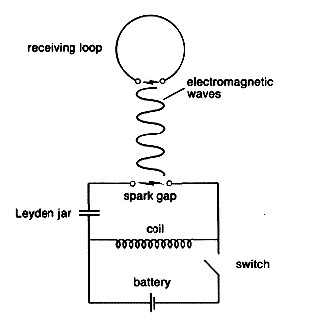
\includegraphics[width=6cm]{hertz_1.jpg}\\
While this diagram shows more detail than required, he found that:
\begin{itemize}
\item Radio waves were produced when a spark lept between the spark balls across an induction coil
\item These radio waves passed through the conductive loop, inducing an EMF across the loop which caused sparks to leap across the spark balls across the ring.
\end{itemize}
Hertz demonstrated that the waves couldn't pass through metal, as the sparks stopped when a metal sheet was placed in front of the ring. He then realised that the metal sheet reflects the waves, as a concave metal sheet behind the source increased the number of sparks across the ring due to more waves being reflected back towards the ring. Hertz also illustrated that the waves pass straight through insulating materials.
\subsection{Measurement of wavelength}
Hertz created standing waves by using a metal sheet to reflect waves back to the source. He moved the detector along a line from the source to the sheet, and observed nodes and antinodes. He calculated the distance between the nodes to be 33cm, meaning that the wavelength must be 66cm.
\subsection{Demonstration of polarity}
Hertz created a reflector that could focus radio waves onto a detector such that the oscillating electric fields creates an alternating pd across the detector, creating sparks at the spark plug. He discovered that when the detector was parallel to the spark gap of the source he obtained a strong signal, which reduced to 0 once the detector had been rotated $90\degree$. This implies that the waves created were polarised - at $90\degree$ the plane of the oscillating electric field was perpendicular to the detector aerials, and no alternating pd was induced.
\section{Fizeau's determination of the speed of light and its implications}
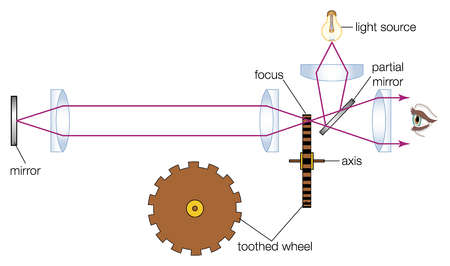
\includegraphics[width=8cm]{fizeau.JPG}\\
Fizeau’s experiment involved using a cog wheel rotating at high speeds while a narrow beam was directed parallel to the axis of the wheel so that it could pass through the gaps between teeth as the wheel rotated.\\
\\
This meant successive teeth and gaps would therefore chop the beam into pulses of light which then travelled to a distant mirror and were reflected back. If the observer could see the reflected light then it meant that the pulses of light were returning back through a gap.\\
\\
Fizeau increased the rotation frequency of the cog wheel from rest until the reflected light could not be seen, calling this frequency $f_0$. At this frequency the time taken for each pulse to travel from the wheel to the mirror and return (a distance equal to 2D, where D equals the distance between the wheel and the mirror) would be equal to the time, t, taken for a gap to be replaced by a tooth.
\newpage
Time for one rotation:
$$T=\frac{1}{f_0}$$
Time for the wheel to move one tooth, where n is the number of teeth
$$t=\frac{T}{2N}$$
Combine the two above equations
$$t=\frac{1}{2f_0N}$$
Apply $\textrm{Speed}=\frac{\textrm{Distance}}{\textrm{Time}}$
$$c=\frac{2D}{\frac{1}{2f_0N}}=4Df_0N$$
\\
Fizeau had a 720 toothed wheel 8633m away from the mirror and found $f_0$ to be equal to 12.6Hz, giving a value of 313,000 $\textrm{kms}^{-1}$ for the speed of light.\\
Fizeau’s determination of the speed of light was important because it was the first terrestrial method of finding the speed of light and was markedly more precise than the previous speed of light found by Ole Rømer (240,000 km/s). It was the first terrestrial method to confirm the speed of light as finite. Furthermore his value agreed with Maxwell’s theoretical value and hence validated Maxwell’s theory of electromagnetic waves.

\end{document}